\section{吸收边界}
\label{sec:4.4}

包含有正在传播之中的波场的一个体积内的各点常常是用计算机内存单元来模拟,虽然
我们往往希望能模拟无限大的体积,可计算机内存单元数令人遗憾地却是有限的。当我们指
望波已传播远去趋向无限远时,计算机内的波却从有限计算机内存所形成之边界反射回来
了。为避免需要计算机有无限大存贮容量,本章建立了有关吸收边界条件的理论。

这里有两类边界困难,第一是要搞清楚在我们的观测终止时我们究竟是处于何处,第二
是我们在何处已设法限制了我们的计算范围。这些边界也许就是同一个边界,但是,为了避
免矛盾,让我们假设数据是具有比计算机内存更为有限的范围,所以同构成计算所需初始条
件的数据在一起的是个将称之为数据补值(data padding)的区域。

\subsection{数据补值}
\label{sec:4.4.1}

最原始的假设是补值区域可设想成是附加的零值数据。为避免边棱绕射这种假象,必须
使数据平滑地与补值相合,因而仅当边界周围的数据已经很小时,补零的办法才是一个很好
的假设。在数据是用零值填补时,是否应作斜坡衰减(逐渐变为零值)使之与填补零值平滑
地匹配起来,这是个可争论的问题。我是宁愿避免对数据采用斜坡衰减处理的,那种办法等
于是窜改歪曲数据。相反,我倒是愿意不用零值来填补数据,而是用看起来有点更像是该数
据的数值来填补。有一种简单的方法就是重复最后的记录道,使它随着远离边界而逐渐衰减
下去,当数据的时差同延长部分的时差能匹配时,这种办法最为有效。任何有关最优数据补
值的理论都具有两个重要组成部分:一个是干扰模型,一个是信号模型。理想的数据外推方
法简直很少能在实践中有效应用。\ref{sec:3.5}节内包含有一些有关于扩展道集的更精细模型的建议。


\subsection{排列端点与测线端点上的截断影响 }
\label{sec:4.4.2}

在勘探中,存在两类水平截断问题。第一类是在排列端点上的截断,它主要影响共中心
点叠加;第二类是在测线的地理边界上的截断,它主要影响偏移。不论在偏移还是叠加中,
都要把双曲面压缩收敛成点,但是两种处理是有区别的,因为数据本身就不同。进行叠加
时,反射能量将倾斜向下移动,有助于形成远炮检距记录道的截断影响是可以断言的。进行
偏移时,反射面在剖面末端上可能是上倾或下倾的,比较好处理的是向下倾斜的情形,地震
同相轴在该处将从边界平滑地移动至剖面内部。

当地震同相轴在测线端点上是上倾时,进行偏移就出现麻烦的情形了,这时向下延拓处
理将地震能量移向了边界。在到达边界的时候它以相反的倾角反跳回来,并与仍然正在继续
移向该边界的地震能量发生了干涉。给时间剖面两侧增添附加空间、从而使倾斜地震能量有
一可去之处,采取这种办法就可以使问题的严重性减小(你事前已经决定把什么初始数据补
值放到这个附加空间中去了)。


\subsection{标量波动方程的Engquist边界}
\label{sec:4.4.3}

最简单的边界条件是这么一种函数,它在边界上应等于零。入射在这样一种边界上的波
以相反的极性被反射回去(所以入射波加反射波会在边界上等于零)。仅次于最简单边界条
件的则是零斜率条件,这也是一种完全反射面,不过反射系数是+1;而不是$-1$
;为代表零斜
率边界,需要在差分网格的边缘端点上有两个点。通常考虑的最一般性边界条件是上述函数
值与斜率的某种线性组合,这种组合也是一种两点式边界条件。事情之所以如此,是因为我
们的各种外推方程(\ref{sec:2.2}节)仅含有单独一个深度方向的导数,所以它们在$z$轴上都是两点式
条件。由于看到了这点,Bjorn
Engquist认识到我们的外推方程可有一种新应用。许多其
他专业领域的研究人员都有兴趣于正演模拟,就是说,以一个像标量波动方程
$P_{xx}+P_{zz}=P_{tt}/v^2$
这样的方程按时间向前推移计算,这些人遇到了计算机内存有限这个严重困难。
Engquist的思想是:他们应该把我们的外推方程用于他们的边界条件(这个思想使他获得
SIAM奖),假设他们希望$(x,z)$空间内的一个方盒子的周围有无限吸收体积。这时,他
们需要环绕方盒子四周有某种边界条件,在盒底部,他们可采用下行波方程;在盒顶部则采
用上行波方程;对于盒的侧面,利用交换$x$与$z$的办法可以作类似的处理,这种思想已由
Robert Clayton作过详尽的试验和证实,他所作各种结果比较之一可作为例子,见图\ref{fig:crft/box}。

\begin{figure}[H]
\centering
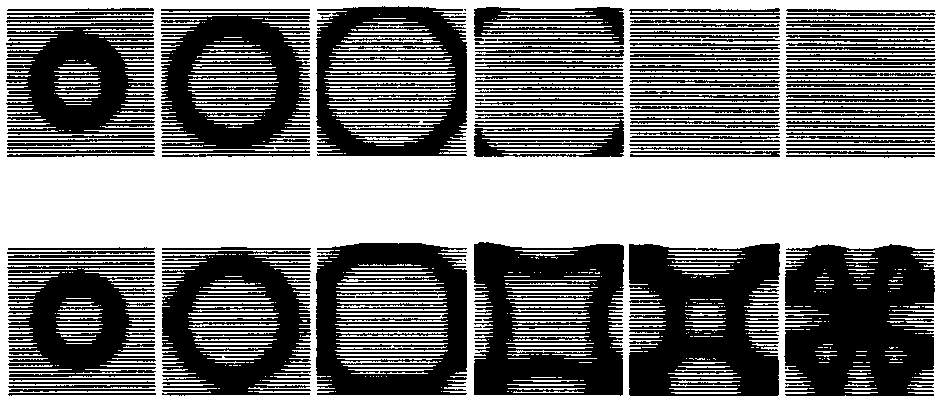
\includegraphics[width=0.65\textwidth]{crft/box}
\caption[box]{在具有吸收边界的盒子内作圆形扩展的波阵面(上图),
在具有零斜率边界的盒子内作圆形扩展的波阵面(下图)(据Clayton)}
\label{fig:crft/box}
\end{figure}

\subsection{外推方程的Engquist侧边条件}
\label{sec:4.4.4}

在数据处理中,是在所研究区域的内部采用外推方程,这点不同于正演模拟问题。在正
演问题中是在所研究区域内部采用完整的标量波动方程,因而在边界上可以采用外推方程。
标量波动方程的波散关系曲线是圆形,而外推方程所具有的理想波散关系曲线却是半圆形。
根据类比推理,Engquist曾推测出,对于波场外推问题,具有四分之一圆弧形的波散关系可
能是一种理想侧边条件。为使他的思想更具体化并能直接应用,他提出用一条直线来近似该
四分之一的圆弧,如图\ref{fig:crft/disperside}所示。

\begin{figure}[H]
\centering
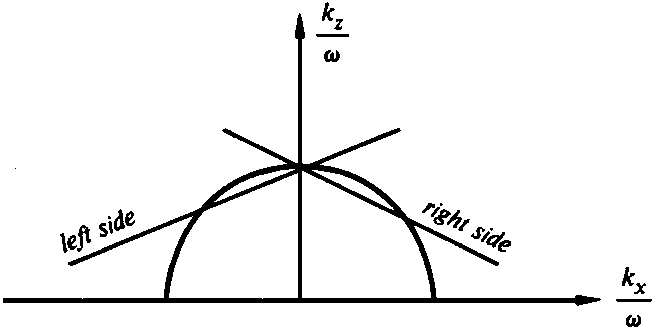
\includegraphics[width=0.65\textwidth]{crft/disperside}
\caption[disperside]{简单吸收侧边界条件的波散关系}
\label{fig:crft/disperside}
\end{figure}

直线形波散关系的好处是在空间域内可用
一个简单的一阶微分方程代表。一阶方程具有
可以只用两个数据点表达的一阶导数,从而可
用于常规的两点式侧边界条件。图\ref{fig:crft/disperside}中的
右侧直线方程定义的边界波散关系D为
\begin{equation}
D(\omega,k_x,k_z)=\frac{vk_z}{\omega}-1+\text{常数}\times \frac{k_x}{\omega}=0
\label{eq:ex4.4.1}
\end{equation}

在$(t,x,z)$空间内,这个方程就是
\begin{equation}
(v\frac{\partial}{\partial z}+
\frac{\partial}{\partial t}+
\text{常数}\frac{\partial}{\partial x})P=0
\label{eq:ex4.4.2}
\end{equation}

若以延迟时间函数形式表示,则在由$(\omega,k_x,k_z)$域变换至$(t,x,z)$域时, $\frac{\partial}{\partial z}$够消去。

就纯数学的而非物理的观点考虑,试想像有某种特定的物理过程,它限定了在某个区域
内可应用的物理方程正就是具有吸收侧边界条件波散关系的方程。除这个虚构的区域以外,
再想像有另一个在其中可应用通常之外推方程的区域。在两个区域的接触点上,方程的解将
符合一致,由此无疑能得出结论:最小的边界反射将出现于两种波散关系彼此良好匹配之
处.所以,为在所感兴趣的角度范围内形成良好的拟合,应适当选择直线的斜率。偏移进行
期间的侧边界吸收作用的一个例子如图\ref{fig:crft/sideabsorb}所示。

\begin{figure}[H]
\centering
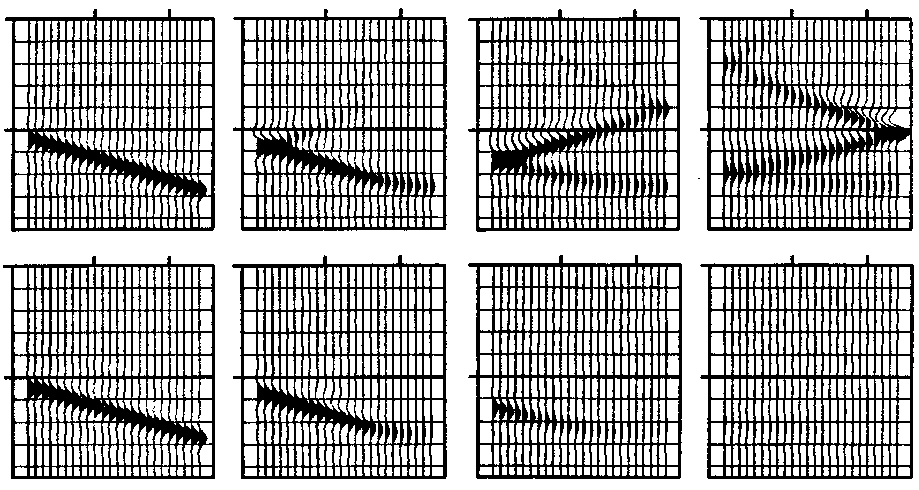
\includegraphics[width=0.65\textwidth]{crft/sideabsorb}
\caption[sideabsorb]{具有零斜率侧边界(上图)和吸收侧边界(下图)
的向下延拓(据Toldi)}
\label{fig:crft/sideabsorb}
\end{figure}

\subsection{反射系数的量值}
\label{sec:4.4.5}

现在让我们考察一下计算反射系数的某些细节,单位振幅的单频平面波入射在侧边界
上,产生幅度为$c$的一个反射波,其数学表现形式为
\begin{equation}
P(x,z)=e^{-i\omega t+ik_zz}(e^{+ik_xx}+ce^{-ik_xx})
\label{eq:ex4.4.3}
\end{equation}
式\ref{eq:ex4.4.3}中的频率$\omega$与水平波数$k_x$都是任意的,而垂直波数$k_z$则是利用内部区域的波散
关系、即半圆近似,根据$\omega$与$k_x$来确定的。假设在侧边界上可应用这种内部解,这时你可将
式\ref{eq:ex4.4.3}代入代表侧边界的微分方程\ref{eq:ex4.4.2}内。结果,在入射波方面,$\partial/\partial x$
转换为$+ik_x$;在反射波方面,$\frac{\partial}{\partial x}$转换为$-ik_x$。还有,$\partial/\partial z$被转换为$ik_z$。因而,式\ref{eq:ex4.4.3}中
的第一项就是波散关系$D(\omega,k_x,k_z)$乘以振幅$P$,第二项等于反射系数c乘$D(\omega,-k_x,k_z)$
再乘$P$。所以,用式\ref{eq:ex4.4.3}代入以后,式\ref{eq:ex4.4.2}就变为
\begin{equation}
c=\frac{-D(\omega,k_x,k_z)}{D(\omega,-k_x,k_z)}
\label{eq:ex4.4.4}
\end{equation}

当根据$\omega,k_x$点上之内部方程所选取的$k_z$数值恰好也准确满足侧边界条件的波散关
系$D$的时候,发生了零反射的情形,这个结果说明了为什么我们要尽可能紧密地与四分之一
圆弧匹配一致,直线型波散关系并不相应于仅可在两个端点上表示的最一般形式之侧边界条
件。有一种具有可调参量$b_8$、$b_2$与$b_1$更一般表达式,它能拟合得甚至更好一点,这种表达式为
\begin{equation*}
D(\omega,k_x,k_z)=(1-b_8\frac{vk_x}{\omega})\frac{vk_z}{\omega}-(b_1-b_2\frac{vk_x}{\omega}
\end{equation*}

对于偏移方程,可以证实直线型吸收侧边界条件是绝对稳定的。可惜,严密的稳定
性分析似乎是超出了
Muir的阻抗规则的理论范围,就是因这个缘故,我是不相信对于45°偏
移方程也已经证实了有稳定性这种说法的。



